% \section{Konzept}
% % \section{Konzept}
% % \section{Konzept}
% % \section{Konzept}
% \input{content/04_erstellung-poc/konzept}

Anhand der Anforderungen und den zuvor in \autoref{sec:werkzeuge-und-technologien} recherchierten Technologien, gilt es nun ein Konzept zu erstellen, wie die Demoanwendung zu erweitern ist. Dabei ist das Grundziel, die Nachvollziehbarkeit dieser Anwendung zu erhöhen. In den Anforderungen werden vier Arten von Daten genannt, die es zu erheben und zu nutzen gilt. Darunter die drei \enquote{Grundpfeiler der Observability} Logs, Metriken und Traces sowie die gesondert zu betrachtende Methodik des Session-Replays.

In \autoref{subsec:bewertung-und-auswahl} wurden kriteriengeleitet bereits Technologien identifiziert, mit denen eine verbesserte Nachvollziehbarkeit erreicht werden kann: Splunk, Sentry, Jaeger sowie LogRocket (vgl. \autoref{tab:uebersicht-ausgewaehlte-technologien}). Bei dieser Übersicht ist zu betrachten, dass Splunk die grundsätzlichen Funktionalitäten von Sentry abdecken kann. Andere Werkzeuge des Error-Monitorings weisen die gleiche Überschneidung auf. Lediglich das Issue-Management, welches in diesen Technologien oft ein fester Bestandteil ist, kann nicht allein mit Splunk abgebildet werden - diese Funktionalität ist aber für die in dieser Arbeit verfolgten Ziele nicht relevant. Weiterhin gehören Bug-Tracking-Systeme bereits unabdingbar zu Softwareprojekten \cite{BugzillaITrackerAndOtherBugTrackers}, ein weiteres ähnlich agierendes System könnte hierbei eine Dopplung darstellen und somit unerwünscht sein. Aus diesem Grund wird auf Sentry verzichtet, dies geht zudem mit der \autoref{anf:3100} einher, welche eine geringe Anzahl an zusätzlichen Partnersystemen vorsieht.

\begingroup
\centering
\setlength{\LTleft}{-20cm plus -1fill}
\setlength{\LTright}{\LTleft}
\begin{longtable}{|p{4.10cm}|p{0.90cm}|p{0.90cm}|p{1.9cm}|p{1.75cm}|p{1.5cm}|p{1.4cm}|p{1.3cm}|}
\hline
Technologie & IM & ASM & RUM & Error-Montoring & Log-Mgmt. & Tracing & Session-Replay \\
\endhead
\hline
Splunk & ja(*) & ja(*) & ja(*) & ja(*) & ja &  &  \\
\hline
Jaeger &  &  &  &  &  & ja &  \\
\hline
Sentry &  &  & ja(*) & ja &  &  &  \\
\hline
LogRocket &  &  & ja & ja &  &  & ja \\
\hline
\caption{Übersicht der ausgewählten Technologien}
\label{tab:uebersicht-ausgewaehlte-technologien}
\end{longtable}
\endgroup

Eine weitere Reduzierung der Anzahl der hinzukommenden Technologien konnte jedoch nicht erreicht werden. Splunk, Jaeger und LogRocket besitzen jeweils Kernfunktionalitäten, die nicht durch andere Werkzeuge abbildbar sind. Splunk ist allen voran ein Log-Management-System, welches durch die Anforderungen erwünscht ist und dabei können die anderen Technologien es nicht ersetzen. Jaeger besitzt mit Distributed-Tracing und LogRocket mit dem Session-Replay in Videoform ebenso Kernfunktionalitäten, die nicht mit anderen Werkzeugen abbildbar sind. Aus diesem Grund soll die Erweiterung auf Basis dieser 3 Technologien erfolgen.

Genauer sollen, wie in \autoref{fig:konzept} visualisiert, aus dem Frontend und den Backend-Diensten Traces erhoben werden und an Jaeger übermittelt werden. Darüber hinaus sind im Frontend Logs, Fehler und Metriken zu erheben und an Splunk zu senden, dabei sind nach Anforderungen \ref*{anf:5220} und \ref*{anf:5410} Fehler und Metriken visuell aufzubereiten.

Zudem sollen über die von LogRocket bereitgestellte JavaScript-Bibliothek die Daten zum Session-Replay erfasst werden und an LogRocket gemeldet werden, jedoch nur wenn der Nutzer zuvor zustimmt (vgl. \autoref{anf:2511}). Splunk und Jaeger sollen zudem lokal, also OnPremise, aufgesetzt werden. LogRocket hingegen bietet dies nur für Unternehmenskunden an und wird somit als SaaS-Produkt zum Einsatz kommen.

Anhand dieses Konzeptes erfolgt im nächsten Abschnitt die Umsetzung dessen. Genauer wird die Implementierung der Erweiterung des Back- und Frontends näher erläutert.

\begin{figure}[H]
	\centering
	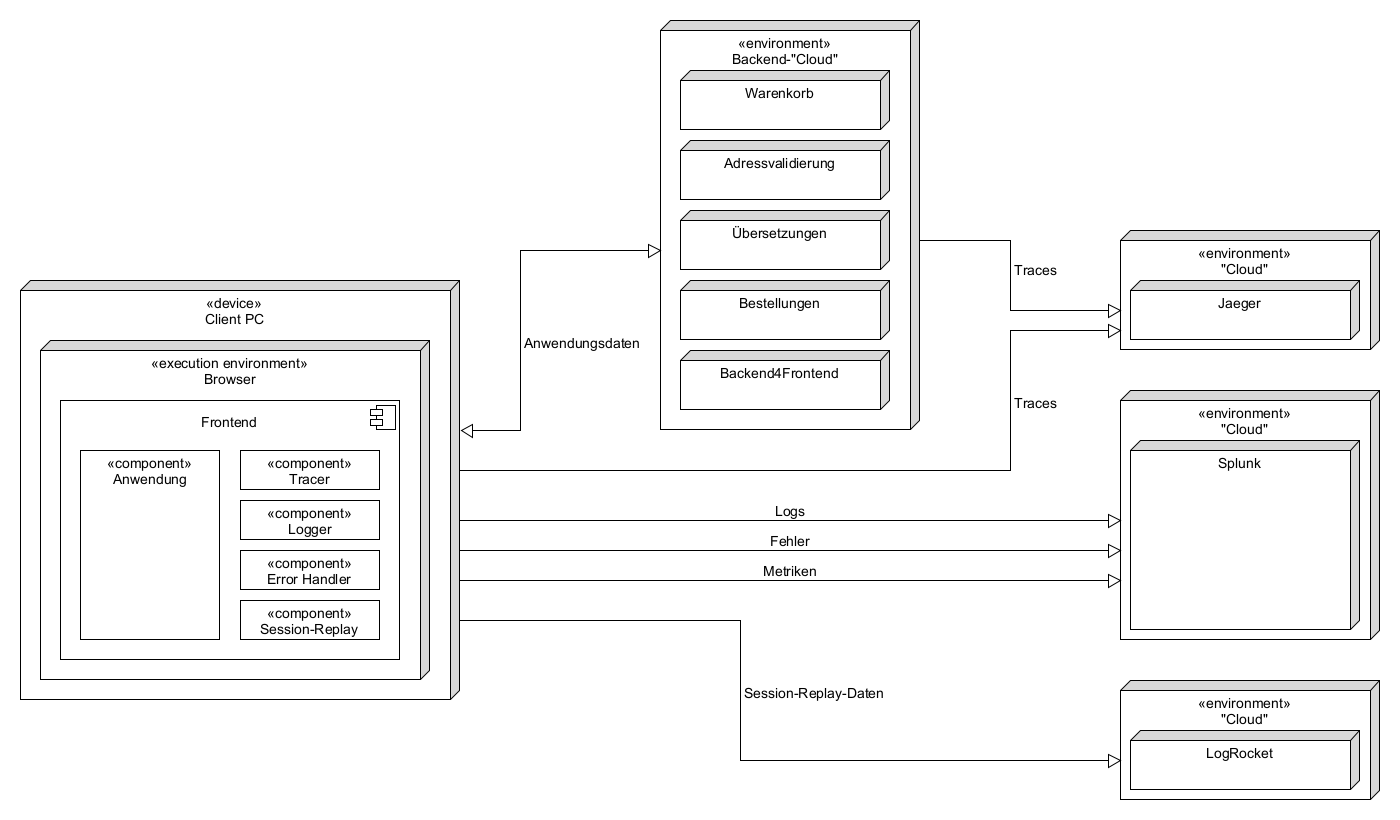
\includegraphics[width=\linewidth]{img/04_erstellung-poc/konzept.png}
	\caption{Architektur des Konzeptes. Eigene Darstellung}
	\label{fig:konzept}
\end{figure}

\vspace{-1\baselineskip}

Anhand der Anforderungen und den zuvor in \autoref{sec:werkzeuge-und-technologien} recherchierten Technologien, gilt es nun ein Konzept zu erstellen, wie die Demoanwendung zu erweitern ist. Dabei ist das Grundziel, die Nachvollziehbarkeit dieser Anwendung zu erhöhen. In den Anforderungen werden vier Arten von Daten genannt, die es zu erheben und zu nutzen gilt. Darunter die drei \enquote{Grundpfeiler der Observability} Logs, Metriken und Traces sowie die gesondert zu betrachtende Methodik des Session-Replays.

In \autoref{subsec:bewertung-und-auswahl} wurden kriteriengeleitet bereits Technologien identifiziert, mit denen eine verbesserte Nachvollziehbarkeit erreicht werden kann: Splunk, Sentry, Jaeger sowie LogRocket (vgl. \autoref{tab:uebersicht-ausgewaehlte-technologien}). Bei dieser Übersicht ist zu betrachten, dass Splunk die grundsätzlichen Funktionalitäten von Sentry abdecken kann. Andere Werkzeuge des Error-Monitorings weisen die gleiche Überschneidung auf. Lediglich das Issue-Management, welches in diesen Technologien oft ein fester Bestandteil ist, kann nicht allein mit Splunk abgebildet werden - diese Funktionalität ist aber für die in dieser Arbeit verfolgten Ziele nicht relevant. Weiterhin gehören Bug-Tracking-Systeme bereits unabdingbar zu Softwareprojekten \cite{BugzillaITrackerAndOtherBugTrackers}, ein weiteres ähnlich agierendes System könnte hierbei eine Dopplung darstellen und somit unerwünscht sein. Aus diesem Grund wird auf Sentry verzichtet, dies geht zudem mit der \autoref{anf:3100} einher, welche eine geringe Anzahl an zusätzlichen Partnersystemen vorsieht.

\begingroup
\centering
\setlength{\LTleft}{-20cm plus -1fill}
\setlength{\LTright}{\LTleft}
\begin{longtable}{|p{4.10cm}|p{0.90cm}|p{0.90cm}|p{1.9cm}|p{1.75cm}|p{1.5cm}|p{1.4cm}|p{1.3cm}|}
\hline
Technologie & IM & ASM & RUM & Error-Montoring & Log-Mgmt. & Tracing & Session-Replay \\
\endhead
\hline
Splunk & ja(*) & ja(*) & ja(*) & ja(*) & ja &  &  \\
\hline
Jaeger &  &  &  &  &  & ja &  \\
\hline
Sentry &  &  & ja(*) & ja &  &  &  \\
\hline
LogRocket &  &  & ja & ja &  &  & ja \\
\hline
\caption{Übersicht der ausgewählten Technologien}
\label{tab:uebersicht-ausgewaehlte-technologien}
\end{longtable}
\endgroup

Eine weitere Reduzierung der Anzahl der hinzukommenden Technologien konnte jedoch nicht erreicht werden. Splunk, Jaeger und LogRocket besitzen jeweils Kernfunktionalitäten, die nicht durch andere Werkzeuge abbildbar sind. Splunk ist allen voran ein Log-Management-System, welches durch die Anforderungen erwünscht ist und dabei können die anderen Technologien es nicht ersetzen. Jaeger besitzt mit Distributed-Tracing und LogRocket mit dem Session-Replay in Videoform ebenso Kernfunktionalitäten, die nicht mit anderen Werkzeugen abbildbar sind. Aus diesem Grund soll die Erweiterung auf Basis dieser 3 Technologien erfolgen.

Genauer sollen, wie in \autoref{fig:konzept} visualisiert, aus dem Frontend und den Backend-Diensten Traces erhoben werden und an Jaeger übermittelt werden. Darüber hinaus sind im Frontend Logs, Fehler und Metriken zu erheben und an Splunk zu senden, dabei sind nach Anforderungen \ref*{anf:5220} und \ref*{anf:5410} Fehler und Metriken visuell aufzubereiten.

Zudem sollen über die von LogRocket bereitgestellte JavaScript-Bibliothek die Daten zum Session-Replay erfasst werden und an LogRocket gemeldet werden, jedoch nur wenn der Nutzer zuvor zustimmt (vgl. \autoref{anf:2511}). Splunk und Jaeger sollen zudem lokal, also OnPremise, aufgesetzt werden. LogRocket hingegen bietet dies nur für Unternehmenskunden an und wird somit als SaaS-Produkt zum Einsatz kommen.

Anhand dieses Konzeptes erfolgt im nächsten Abschnitt die Umsetzung dessen. Genauer wird die Implementierung der Erweiterung des Back- und Frontends näher erläutert.

\begin{figure}[H]
	\centering
	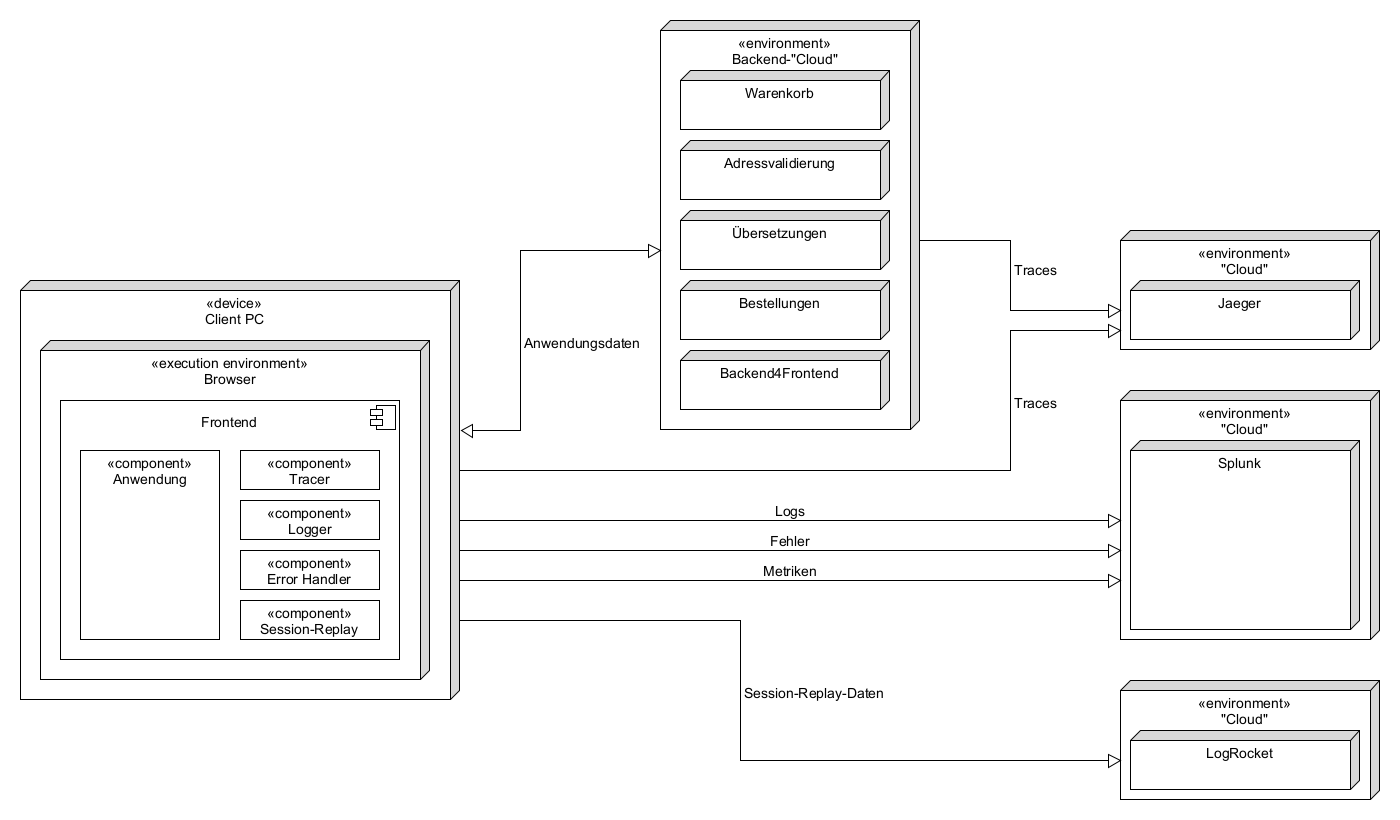
\includegraphics[width=\linewidth]{img/04_erstellung-poc/konzept.png}
	\caption{Architektur des Konzeptes. Eigene Darstellung}
	\label{fig:konzept}
\end{figure}

\vspace{-1\baselineskip}

Anhand der Anforderungen und den zuvor in \autoref{sec:werkzeuge-und-technologien} recherchierten Technologien, gilt es nun ein Konzept zu erstellen, wie die Demoanwendung zu erweitern ist. Dabei ist das Grundziel, die Nachvollziehbarkeit dieser Anwendung zu erhöhen. In den Anforderungen werden vier Arten von Daten genannt, die es zu erheben und zu nutzen gilt. Darunter die drei \enquote{Grundpfeiler der Observability} Logs, Metriken und Traces sowie die gesondert zu betrachtende Methodik des Session-Replays.

In \autoref{subsec:bewertung-und-auswahl} wurden kriteriengeleitet bereits Technologien identifiziert, mit denen eine verbesserte Nachvollziehbarkeit erreicht werden kann: Splunk, Sentry, Jaeger sowie LogRocket (vgl. \autoref{tab:uebersicht-ausgewaehlte-technologien}). Bei dieser Übersicht ist zu betrachten, dass Splunk die grundsätzlichen Funktionalitäten von Sentry abdecken kann. Andere Werkzeuge des Error-Monitorings weisen die gleiche Überschneidung auf. Lediglich das Issue-Management, welches in diesen Technologien oft ein fester Bestandteil ist, kann nicht allein mit Splunk abgebildet werden - diese Funktionalität ist aber für die in dieser Arbeit verfolgten Ziele nicht relevant. Weiterhin gehören Bug-Tracking-Systeme bereits unabdingbar zu Softwareprojekten \cite{BugzillaITrackerAndOtherBugTrackers}, ein weiteres ähnlich agierendes System könnte hierbei eine Dopplung darstellen und somit unerwünscht sein. Aus diesem Grund wird auf Sentry verzichtet, dies geht zudem mit der \autoref{anf:3100} einher, welche eine geringe Anzahl an zusätzlichen Partnersystemen vorsieht.

\begingroup
\centering
\setlength{\LTleft}{-20cm plus -1fill}
\setlength{\LTright}{\LTleft}
\begin{longtable}{|p{4.10cm}|p{0.90cm}|p{0.90cm}|p{1.9cm}|p{1.75cm}|p{1.5cm}|p{1.4cm}|p{1.3cm}|}
\hline
Technologie & IM & ASM & RUM & Error-Montoring & Log-Mgmt. & Tracing & Session-Replay \\
\endhead
\hline
Splunk & ja(*) & ja(*) & ja(*) & ja(*) & ja &  &  \\
\hline
Jaeger &  &  &  &  &  & ja &  \\
\hline
Sentry &  &  & ja(*) & ja &  &  &  \\
\hline
LogRocket &  &  & ja & ja &  &  & ja \\
\hline
\caption{Übersicht der ausgewählten Technologien}
\label{tab:uebersicht-ausgewaehlte-technologien}
\end{longtable}
\endgroup

Eine weitere Reduzierung der Anzahl der hinzukommenden Technologien konnte jedoch nicht erreicht werden. Splunk, Jaeger und LogRocket besitzen jeweils Kernfunktionalitäten, die nicht durch andere Werkzeuge abbildbar sind. Splunk ist allen voran ein Log-Management-System, welches durch die Anforderungen erwünscht ist und dabei können die anderen Technologien es nicht ersetzen. Jaeger besitzt mit Distributed-Tracing und LogRocket mit dem Session-Replay in Videoform ebenso Kernfunktionalitäten, die nicht mit anderen Werkzeugen abbildbar sind. Aus diesem Grund soll die Erweiterung auf Basis dieser 3 Technologien erfolgen.

Genauer sollen, wie in \autoref{fig:konzept} visualisiert, aus dem Frontend und den Backend-Diensten Traces erhoben werden und an Jaeger übermittelt werden. Darüber hinaus sind im Frontend Logs, Fehler und Metriken zu erheben und an Splunk zu senden, dabei sind nach Anforderungen \ref*{anf:5220} und \ref*{anf:5410} Fehler und Metriken visuell aufzubereiten.

Zudem sollen über die von LogRocket bereitgestellte JavaScript-Bibliothek die Daten zum Session-Replay erfasst werden und an LogRocket gemeldet werden, jedoch nur wenn der Nutzer zuvor zustimmt (vgl. \autoref{anf:2511}). Splunk und Jaeger sollen zudem lokal, also OnPremise, aufgesetzt werden. LogRocket hingegen bietet dies nur für Unternehmenskunden an und wird somit als SaaS-Produkt zum Einsatz kommen.

Anhand dieses Konzeptes erfolgt im nächsten Abschnitt die Umsetzung dessen. Genauer wird die Implementierung der Erweiterung des Back- und Frontends näher erläutert.

\begin{figure}[H]
	\centering
	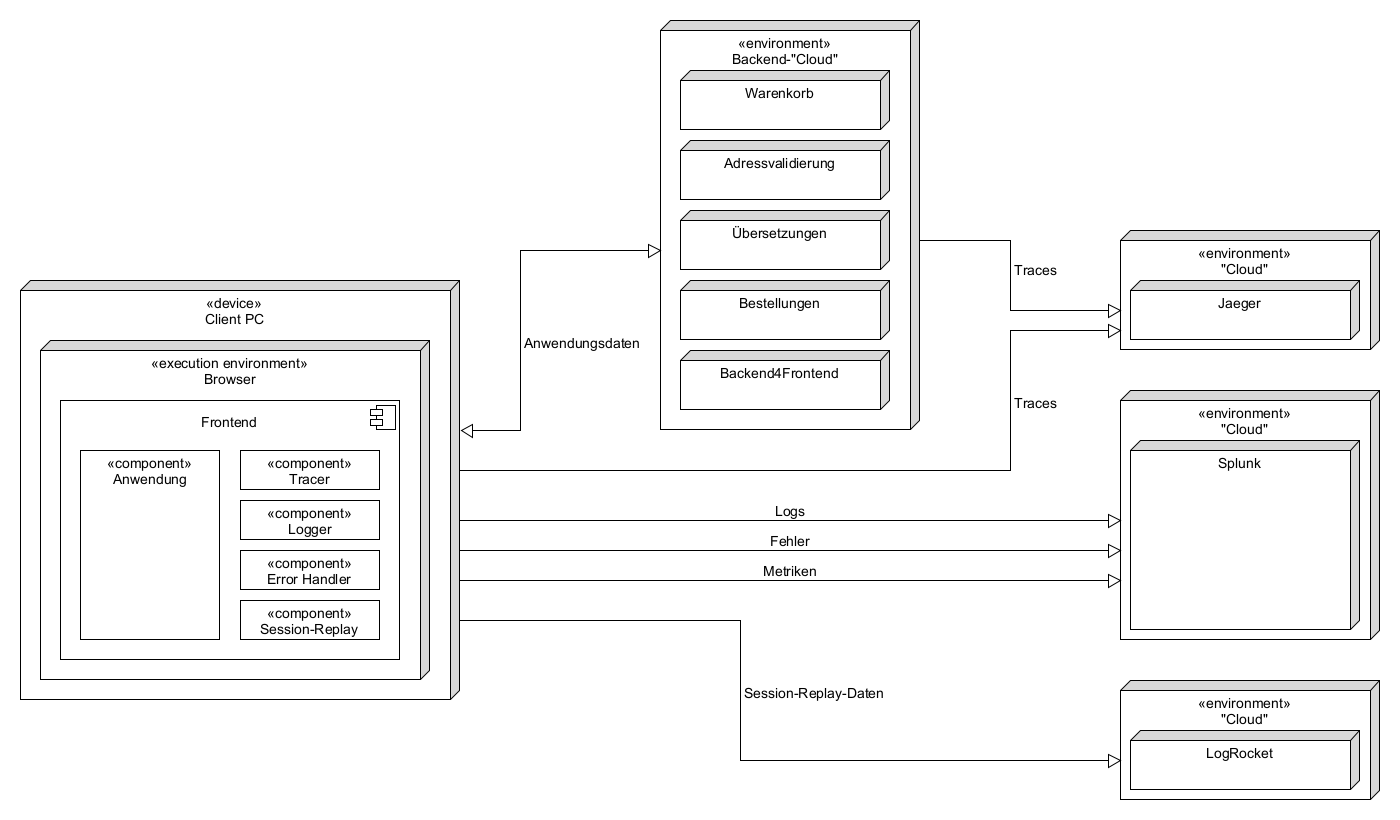
\includegraphics[width=\linewidth]{img/04_erstellung-poc/konzept.png}
	\caption{Architektur des Konzeptes. Eigene Darstellung}
	\label{fig:konzept}
\end{figure}

\vspace{-1\baselineskip}

Anhand der Anforderungen und den zuvor in \autoref{sec:werkzeuge-und-technologien} recherchierten Technologien, gilt es nun ein Konzept zu erstellen, wie die Demoanwendung zu erweitern ist. Dabei ist das Grundziel, die Nachvollziehbarkeit dieser Anwendung zu erhöhen. In den Anforderungen werden 4 Arten von Daten genannt, die es zu erheben und zu nutzen gilt. Darunter die 3 \enquote{Grundpfeiler der Observability} Logs, Metriken und Traces sowie die gesondert zu betrachtende Methodik des Session-Replays.

In \autoref{subsec:bewertung-und-auswahl} wurden kriteriengeleitet bereits Technologien identifiziert, mit denen eine verbesserte Nachvollziehbarkeit erreicht werden kann: Splunk, Sentry, Jaeger sowie LogRocket (vgl. \autoref{tab:uebersicht-ausgewaehlte-technologien}). Bei dieser Übersicht ist zu betrachten, dass Splunk die grundsätzlichen Funktionalitäten von Sentry abdecken kann. Andere Werkzeuge des Error-Monitorings weisen die gleiche Überschneidung auf. Lediglich das Issue-Management, welches in diesen Technologien oft ein fester Bestandteil ist, kann nicht allein mit Splunk abgebildet werden - diese Funktionalität ist aber für die in dieser Arbeit verfolgten Ziele nicht relevant. Weiterhin gehören Bug-Tracking-Systeme bereits unabdingbar zu Softwareprojekten \cite{BugzillaITrackerAndOtherBugTrackers}, ein weiteres ähnlich agierendes System könnte hierbei eine Dopplung darstellen und somit unerwünscht sein. Aus diesem Grund wird auf Sentry verzichtet, dies geht zudem mit der \autoref{anf:3100} einher, welche eine geringe Anzahl an zusätzlichen Partnersystemen vorsieht.

\begingroup
\centering
\setlength{\LTleft}{-20cm plus -1fill}
\setlength{\LTright}{\LTleft}
\begin{longtable}{|p{4.10cm}|p{0.90cm}|p{0.90cm}|p{1.9cm}|p{1.75cm}|p{1.5cm}|p{1.4cm}|p{1.3cm}|}
\hline
Technologie & IM & ASM & RUM & Error-Montoring & Log-Mgmt. & Tracing & Session-Replay \\
\endhead
\hline
Splunk & ja(*) & ja(*) & ja(*) & ja(*) & ja &  &  \\
\hline
Jaeger &  &  &  &  &  & ja &  \\
\hline
Sentry &  &  & ja(*) & ja &  &  &  \\
\hline
LogRocket &  &  & ja & ja &  &  & ja \\
\hline
\caption{Übersicht der ausgewählten Technologien}
\label{tab:uebersicht-ausgewaehlte-technologien}
\end{longtable}
\endgroup

Weitere Abdeckungen einer Technologie durch eine andere lassen sich jedoch nicht feststellen, Splunk, Jaeger sowie LogRocket besitzen jeweils Kernfunktionalitäten, die nicht durch andere Werkzeuge abbildbar sind. Splunk ist allen voran ein Log-Management-System und in dieser Funktion mit den anderen Technologien nicht ersetzbar. Jaeger besitzt mit Distributed-Tracing und LogRocket mit dem Session-Replay in Videoform ebenso Kernfunktionalitäten, die nicht mit anderen Werkzeugen abbildbar sind. Aus diesem Grund soll die Erweiterung auf Basis dieser 3 Technologien erfolgen.

Genauer sollen, wie in \autoref{fig:konzept} visualisiert, aus dem Frontend und den Backend-Diensten Tracedaten erhoben werden und an Jaeger übermittelt werden. Darüber hinaus sind im Frontend Logs, Fehler und Metriken zu erheben und an Splunk zu senden, dabei sind nach Anforderungen \ref*{anf:5220} und \ref*{anf:5410} Fehler und Metriken visuell aufzubereiten. Zudem sollen über die von LogRocket bereitgestellte JavaScript-Bibliothek die Daten zum Session-Replay erfasst werden und an LogRocket gemeldet werden, jedoch nur wenn der Nutzer zuvor zustimmt (vgl. \autoref{anf:2511}). Splunk und Jaeger sollen zudem lokal, also OnPremise, aufgesetzt werden. LogRocket hingegen bietet dies nur für Unternehmenskunden an und wird somit als SaaS-Produkt zum Einsatz kommen.

Auf dieser Basis erfolgt im nächsten Abschnitt die Implementierung der Erweiterung sowie die Umsetzung des Konzeptes. Hierbei werden die notwendigen Schritte technisch erläutert, eine nicht technische Übersicht erfolgt hingegen in \autoref{sec:demonstration}.

\begin{figure}[H]
	\centering
	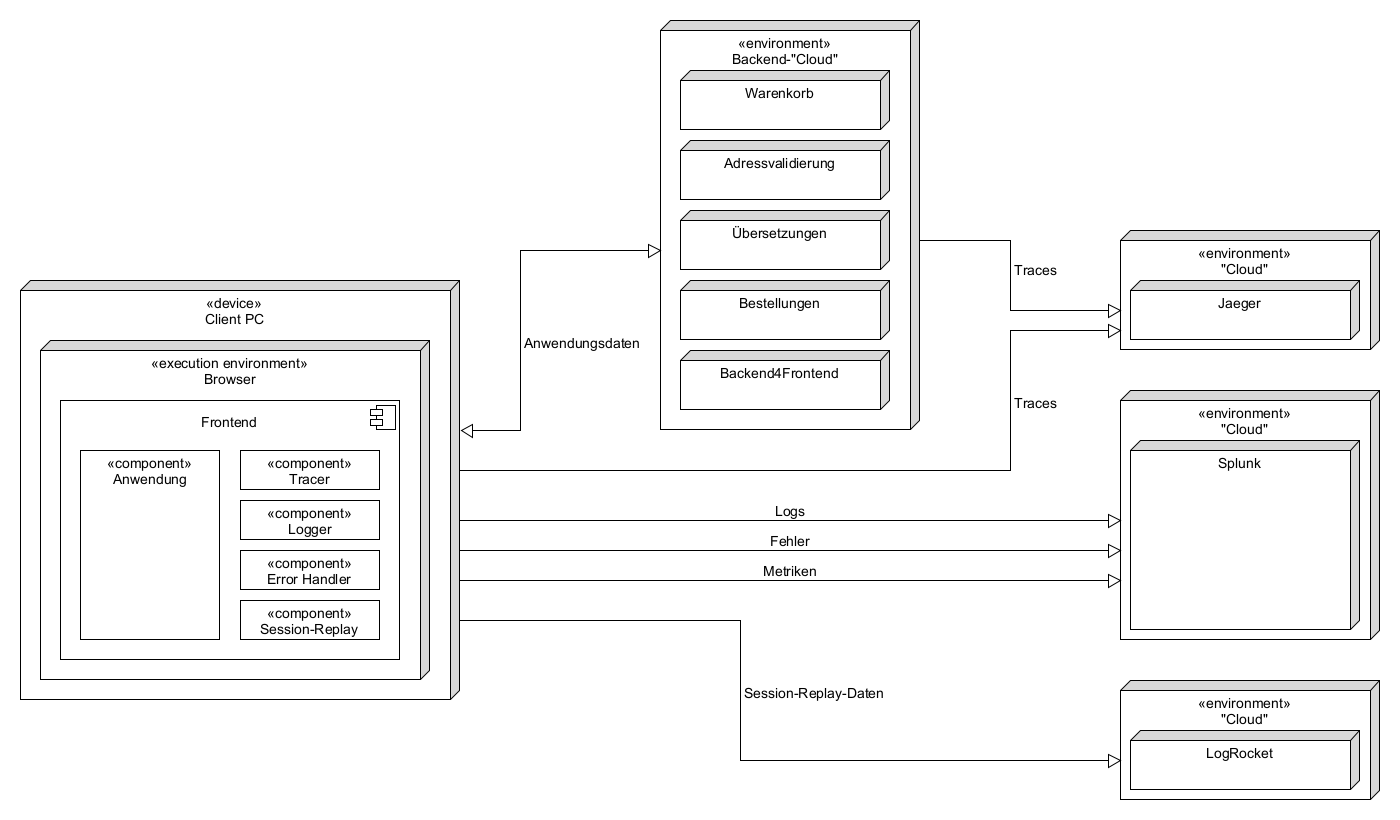
\includegraphics[width=\linewidth]{img/04_erstellung-poc/konzept.png}
	\caption{Architektur des Konzeptes. Eigene Darstellung}
	\label{fig:konzept}
\end{figure}

\vspace{-1\baselineskip}